%
% fastalgo.tex -- Data flow for fast algorithm
%
% (c) 2019 Prof Dr Andreas Müller, Hochschule Rapperswil
%
\documentclass[tikz]{standalone}
\usepackage{amsmath}
\usepackage{times}
\usepackage{txfonts}
\usepackage{pgfplots}
\usepackage{csvsimple}
\usetikzlibrary{arrows,intersections,math}
\begin{document}
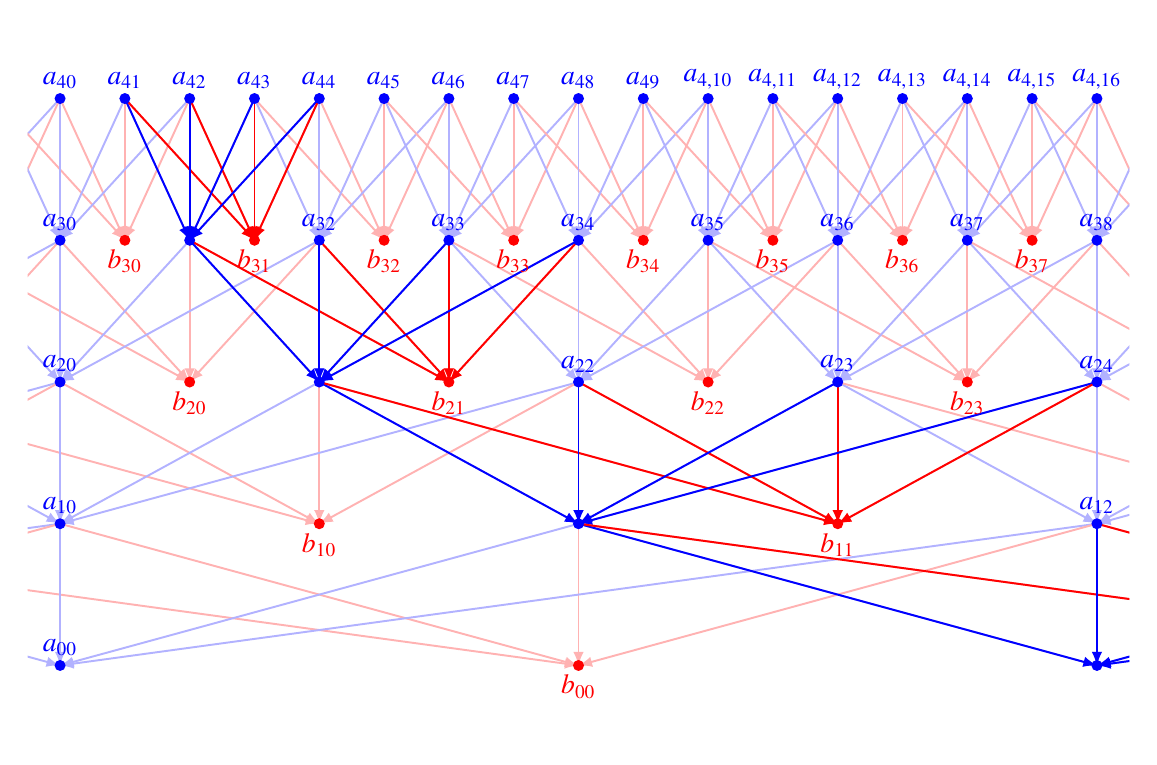
\begin{tikzpicture}[>=latex]

\def\s{0.823}
\def\t{1.8}
\def\r{0.07}

\begin{scope}
\clip ({-0.5*\s},{-2.5*\t}) rectangle ({16.5*\s},{2.5*\t});

\foreach \x in {-2,0,...,16}{
	\foreach \k in {-1,...,2}{
		\draw[->,color=blue!30,line width=0.7pt]
			({(\x+\k)*\s},{2*\t})--({\x*\s},{1*\t});
		\draw[->,color=red!30,line width=0.7pt]
			({(\x+\k)*\s},{2*\t})--({(\x+1)*\s},{1*\t});
	}
}
\xdef\x{2}
\foreach \k in {-1,...,2}{
	\draw[->,color=blue,line width=0.7pt]
		({(\x+\k)*\s},{2*\t})--({\x*\s},{1*\t});
	\draw[->,color=red,line width=0.7pt]
		({(\x+\k)*\s},{2*\t})--({(\x+1)*\s},{1*\t});
}

\foreach \x in {-4,0,4,8,12,16}{
	\foreach \k in {-1,...,2}{
		\draw[->,color=blue!30,line width=0.7pt]
			({(\x+2*\k)*\s},{1*\t})--({\x*\s},{0*\t});
		\draw[->,color=red!30,line width=0.7pt]
			({(\x+2*\k)*\s},{1*\t})--({(\x+2)*\s},{0*\t});
	}
}
\xdef\x{4}
\foreach \k in {-1,...,2}{
	\draw[->,color=blue,line width=0.7pt]
		({(\x+2*\k)*\s},{1*\t})--({\x*\s},{0*\t});
	\draw[->,color=red,line width=0.7pt]
		({(\x+2*\k)*\s},{1*\t})--({(\x+2)*\s},{0*\t});
}

\foreach \x in {-8,0,8,16}{
	\foreach \k in {-1,...,2}{
		\draw[->,color=blue!30,line width=0.7pt]
			({(\x+4*\k)*\s},{0*\t})--({\x*\s},{-1*\t});
		\draw[->,color=red!30,line width=0.7pt]
			({(\x+4*\k)*\s},{0*\t})--({(\x+4)*\s},{-1*\t});
	}
}
\xdef\x{8}
\foreach \k in {-1,...,2}{
	\draw[->,color=blue,line width=0.7pt]
		({(\x+4*\k)*\s},{0*\t})--({\x*\s},{-1*\t});
	\draw[->,color=red,line width=0.7pt]
		({(\x+4*\k)*\s},{0*\t})--({(\x+4)*\s},{-1*\t});
}

\foreach \x in {-16,0,16}{
	\foreach \k in {-1,...,2}{
		\draw[->,color=blue!30,line width=0.7pt]
			({(\x+8*\k)*\s},{-1*\t})--({\x*\s},{-2*\t});
		\draw[->,color=red!30,line width=0.7pt]
			({(\x+8*\k)*\s},{-1*\t})--({(\x+8)*\s},{-2*\t});
	}
}
\xdef\x{16}
\foreach \k in {-1,...,2}{
	\draw[->,color=blue,line width=0.7pt]
		({(\x+8*\k)*\s},{-1*\t})--({\x*\s},{-2*\t});
	\draw[->,color=red,line width=0.7pt]
		({(\x+8*\k)*\s},{-1*\t})--({(\x+8)*\s},{-2*\t});
}



\foreach \x in {-2,...,16}{
	\fill[color=blue] ({\x*\s},{2*\t}) circle[radius={\r}];
}

\foreach \x in {-2,0,...,16}{
	\fill[color=blue] ({\x*\s},{1*\t}) circle[radius={\r}];
	\fill[color=red] ({(\x+1)*\s},{1*\t}) circle[radius={\r}];
}

\foreach \x in {0,4,...,16}{
	\fill[color=blue] ({\x*\s},{0*\t}) circle[radius={\r}];
	\fill[color=red] ({(\x+2)*\s},{0*\t}) circle[radius={\r}];
}

\foreach \x in {-8,0,8,16}{
	\fill[color=blue] ({\x*\s},{-1*\t}) circle[radius={\r}];
	\fill[color=red] ({(\x+4)*\s},{-1*\t}) circle[radius={\r}];
}

\foreach \x in {-16,0,16}{
	\fill[color=blue] ({\x*\s},{-2*\t}) circle[radius={\r}];
	\fill[color=red] ({(\x+8)*\s},{-2*\t}) circle[radius={\r}];
}

\foreach \k in {0,...,9}{
	\node[color=blue] at ({\k*\s},{2*\t}) [above] {$a_{4\k}$};
}
\foreach \k in {10,...,16}{
	\node[color=blue] at ({\k*\s},{2*\t}) [above] {$a_{4,\k}$};
}


\node[color=blue] at ({0*\s},{1*\t}) [above] {$a_{30}$};
\node[color=red] at ({1*\s},{1*\t}) [below] {$b_{30}$};
\node[color=red] at ({3*\s},{1*\t}) [below] {$b_{31}$};
\foreach \k in {2,...,8}{
	\node[color=blue] at ({2*\k*\s},{1*\t}) [above] {$a_{3\k}$};
	\node[color=red] at ({(2*\k+1)*\s},{1*\t}) [below] {$b_{3\k}$};
}

\node[color=blue] at ({0*\s},{0*\t}) [above] {$a_{20}$};
\node[color=red] at ({2*\s},{0*\t}) [below] {$b_{20}$};
\node[color=red] at ({6*\s},{0*\t}) [below] {$b_{21}$};
\foreach \k in {2,...,8}{
	\node[color=blue] at ({2*\k*2*\s},{0*\t}) [above] {$a_{2\k}$};
	\node[color=red] at ({(2*\k+1)*2*\s},{0*\t}) [below] {$b_{2\k}$};
}

\node[color=blue] at ({0*\s},{-1*\t}) [above] {$a_{10}$};
\node[color=red] at ({4*\s},{-1*\t}) [below] {$b_{10}$};
\node[color=red] at ({12*\s},{-1*\t}) [below] {$b_{11}$};
\foreach \k in {2,...,8}{
	\node[color=blue] at ({2*\k*4*\s},{-1*\t}) [above] {$a_{1\k}$};
	\node[color=red] at ({(2*\k+1)*4*\s},{-1*\t}) [below] {$b_{1\k}$};
}

\node[color=blue] at ({0*\s},{-2*\t}) [above] {$a_{00}$};
\node[color=red] at ({8*\s},{-2*\t}) [below] {$b_{00}$};
\foreach \k in {2,...,8}{
	\node[color=blue] at ({2*\k*8*\s},{-1*\t}) [above] {$a_{0\k}$};
	\node[color=red] at ({(2*\k+1)*8*\s},{-1*\t}) [below] {$b_{0\k}$};
}

\end{scope}

\end{tikzpicture}
\end{document}

